\documentclass[danish,a4paper,twocolumn,amsmath,amssymb]{revtex4-1}
\usepackage{babel}		%Giver mulighed for dansk orddeling. Slet kun hvis du VED hvad du laver, eller skal skrive noget på engelsk.
\usepackage[latin1]{inputenc}	%Tillader danske tegn
\usepackage[T1]{fontenc}	%Tillader danske tegn
\usepackage{graphicx}		%Tillader indsættelse af billeder
\usepackage{dcolumn}		%Bruges til at lave matematiske tabelsøjler... se datatabel
\usepackage{booktabs}		%linjer i tabeller...
\usepackage{mathtools}		%Ekstra matematik... bare lad den være, du får muligvis brug for den.
\usepackage{multirow}
\usepackage{threeparttable} 			% Jeg kan ikke huske hvad den gør, men den skal bruges til for at tabelnoterne virker
\usepackage[tableposition=top]{caption} % Noget med at lave caption så det står godt
\usepackage[version=3]{mhchem}  %\ce{H2O + e^{-} -> H2O^{+} + 2e^-}
%siunitx-pakken er ny ift. den originale template, så der henvises i tekstan til en anden pakke, beklager.
\usepackage{siunitx}	%Bruges \SI{<tal>}{<enhed>}, \si{<enhed>} eller \num{<tal>}.
\sisetup{output-decimal-marker={,},separate-uncertainty=true}%Sørger for komma som decimalmarkør. Virker også ved decimaltal, hvis man bruger \num{<tal>}.
\usepackage{url}		 %bruges til at formattere url'er... kan sagtens udelades.
%Det følgende laver to makroer, \tref{} og \fref, der kan bruges ligesom \ref til at referere til hhv. tabeller og figurer. 
%De indsætter selv ordet Tabel/Figur, og sørger for at der ikke sker et linjebrud mellem dette og nummeret.
\newcommand{\tref}[1]{\tablename~\ref{#1}}
\newcommand{\fref}[1]{\figurename~\ref{#1}}
%Tilsvarende for ligninger. Indsætter "ligning (#)".
\newcommand{\lref}[1]{ligning~\eqref{#1}}
	% \eqref laver en reference med parenteser omkring (til brug ved ligninger.)

%Disse makroer indsætter ordene "PicoScope" og "EasyPlot" i teksten (med store bogstaver. Husk at sætte "{}" bagefter for at få et mellemrum.
%Jeg har lavet dem fordi jeg blev træt af at sidde og trykke shift hele tiden, og for at få det til at stå ens. Brug dem, eller lad være.
\newcommand{\picos}[0]{\textsc{PicoScope}} %hedder \picos for ikke at komme i kambolage med pico fra SIunits.
\newcommand{\epw}[0]{\textsc{EasyPlot}}    %epw er navnet på programfilen for easyplot, men det har ingen betydning for makroen. Jeg valgte det fordi det var noget jeg kunne huske, og det kan sagtens ændres.
\newcommand{\matl}[0]{\textsc{Matlab}} %Skriver Matlab med small caps.
\usepackage[footnote,draft,english,silent,nomargin]{fixme}
%hyperref-pakken kan bruges til at redigere pdf-metadata. Det kan være et nice touch, men er generelt ikke påkrævet. Laver automatisk referencer i teksten til farvede hyperlinks i.
\usepackage{hyperref}
\hypersetup
{   pdfsubject={Rapport},
	pdfauthor={Alexander Rasborg Knudsen}
    pdftitle={Masse},
    pdfstartview=FitH,
    colorlinks=true}
    
%Følgende gør, at subscripts bliver ikke-kursiv. Anvendes X_|<subscript>|. Erstattes evt. med X_{\mathrm{<subscript>}}.
\makeatletter
\begingroup
\catcode`\_=\active
\protected\gdef_{\@ifnextchar|\subtextup\sb}
\endgroup
\def\subtextup|#1|{\sb{\textup{#1}}}
\AtBeginDocument{\catcode`\_=12 \mathcode`\_=32768 }
\makeatother

\usepackage[danish=quotes]{csquotes} %Danske citationstegn. \enquote{}

%Lad disse to linjer være. De sørger for at bunden af siden bliver pæn, og fjerner indryk ved afsnit.
\raggedbottom
\parindent = 0pt

% A file like this(called home.tex) could be placed in each latex project folder. 

% This will give the possibility to use modules like this:
% % A file like this(called home.tex) could be placed in each latex project folder. 

% This will give the possibility to use modules like this:
% \input{home} - This is needed to use the \home command
% \input{\home/Modules/Usepackages}
% \input{\home/Modules/ChapterStyle}
% \input{\home/Modules/HeaderAndFooter}

% If you use Github or any other collaborating tool, you should ignore the home.tex file, so that every user could have their own home.tex file.

\newcommand{\home}{C:/Users/Alexander/Documents/GitHub/LaTeX} - This is needed to use the \home command
% \input{\home/Modules/Usepackages}
% \input{\home/Modules/ChapterStyle}
% \input{\home/Modules/HeaderAndFooter}

% If you use Github or any other collaborating tool, you should ignore the home.tex file, so that every user could have their own home.tex file.

\newcommand{\home}{C:/Users/Alexander/Documents/GitHub/LaTeX}
%\input{\home/Modules/Usepackages}
%\input{\home/Modules/ChapterStyle}
%\input{\home/Modules/HeaderAndFooter}
%\input{\home/Modules/Paragraph}
\input{\home/Modules/Figure}

%FixMe pakken viser små kommentarer, hvor der skal rettes
%--------------------------------------------------
%Brug med følgende: \fxnote{det her skal uddybes!} 
%Se liste over alle fixMe's: \listoffixmes
%Erstat 'draft' med 'final' for at fjerne alle kommentarer
%--------------------------------------------------
\usepackage[footnote,draft,english,silent,nomargin]{fixme}


\begin{document}
\title{TINONS Project: Speaker recognition}

\author{Kasper Nielsen}%Forfatter 1
\author{Alexander Rasborg Knudsen}%Forfatter 2
\affiliation{Department of Engineering, Aarhus Universitet} 
\date{\today} %Dato.

\begin{abstract}
\bigskip
The principal objective of this paper is finding a speaker classification.
\end{abstract}

\maketitle
\noindent

\section*{Introduction}
assefilter, detektor, data-analysesystem. 
Gassen til analyse suges ind i maskinen gennem et kapillarrr (snifferen), som kan bnes og lukkes med en mekanisk ventil (inlet valve). 
For at mindske risikoen for, at ioner fragmenterer, bliver neutraliseret eller spredt p hinanden, skal kollisionerne imelle
assefilter, detektor, data-analysesystem. 
Gassen til analyse suges ind i maskinen gennem et kapillarrr (snifferen), som kan bnes og lukkes med en mekanisk ventil (inlet valve). 
 
For at mindske risikoen for, at ioner fragmenterer, bliver neutraliseret eller spredt p hinanden, skal kollisionerne imelle \cite{RefWorks:22}

\begin{figure} 
	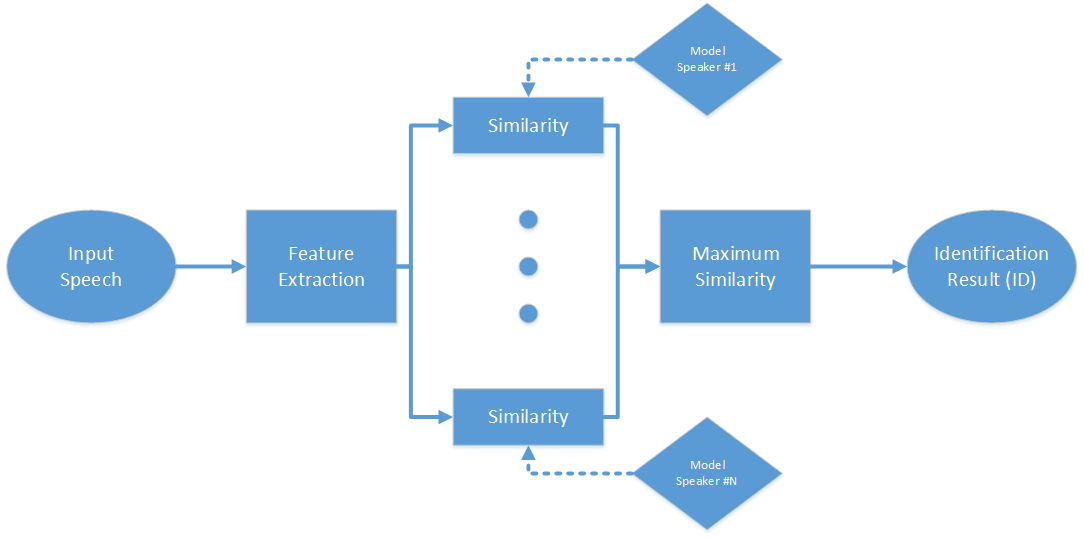
\includegraphics[width=\columnwidth]{Figures/Overview_speech_01.png}
	\caption{\textit{Show an overview of the speaker recognition}}
	\label{fig:Overview}
\end{figure} % DONE ?

\subsection*{Data Collection}

This projects dataset consist of 1.656 sound files. 
Divided into a large training set and a smaller test set. 
Each file is 2 seconds long and was recorded at 48 kHz.
The data structure consist of 4 persons stating a number between 0 to 9. 
The data is borrowed with permission from Christoffer Mose, Simon Madsen, Camilla Munk and Jacob Hansen.
   % DONE ?

%!TEX root = Main.tex
\subsection*{Feature Extraction}
When doing speaker recognition it is advantageous to classify on the basis of extracted features from speech data, rather than the audio samples themselves \cite{Springer:36}.
Features were extracted on a frame-to-frame basis.
This was done on the assumption of pseudo-stationarity of human speech in the scale of a few tens of ms \cite{Springer:36}.
The frames consisted of 256 samples, with a new frame staring every 100 samples.
This means that we have a frame length of
\begin{equation}
t_{frame length} = \dfrac{N_{frame}}{F_s} = \dfrac{256}{48\ kHz} = 5.33\ ms
\end{equation}

and a frame interval of
\begin{equation}
t_{frame interval} = \dfrac{N_{interval}}{F_s} = \dfrac{100}{48\ kHz} = 2.08\ ms
\end{equation}

The features extracted for use in classification were $12^{th}$ order Mel-frequency Cepstral Coefficients (MFCC), as they hava proven effective in speaker regocnition applications and speech processing in general.
Further, so-called delta and double-delta coeffcients, the temporal derivatives $ \frac{dC}{dt} $ and double-derivatives $\frac{d^2C}{dt}$ of the MFCCs respectively, are used as features.
\footnote{For more on MFCC and feature extraction, see Appendix} \fxnote{fix footnotes} % DONE ?

\section*{Classification}

	\subsection*{Linear Classification}
In linear classification the decision surfaces are linear functions of the input vector $\mathbf{x}$.
the target of the classification is labelled in the target variable $\mathbf{t}$, using the target values to represent class labels.
In this project there are 3 different speakers, $K = 3$ then the target vector for class 3 be $\mathbf{t} = (0, 0, 1)^T$.
The value of $t_k$ can be interpreted as the probability of the given class being class $C_k$.
To assign each vector $\mathbf{x}$ with a specific class.
The linear discriminant function in its simplest form
\begin{equation}
y(\mathbf{x}) = \mathbf{w}^T \mathbf{x}+w_0
\label{eq:lin_output}
\end{equation}

\paragraph*{Training}
The linear classifier is applied to the training dataset, containing feature vectors $(\mathbf{x}_n)$ and the target vectors $(\mathbf{t}_n)$.
The vectors are on the form:
\begin{equation}
\mathbf{\tilde{X}}=\left[ \begin{array}{c}\mathbf{x}_1^T \quad 1\\
\mathbf{x}_2^T \quad 1\\
...\\ 
\mathbf{x}_n^T \quad 1 \end{array} \right],
\;
\mathbf{T}=\left[ \begin{array}{c}
\mathbf{t}_1^T\\ 
\mathbf{t}_2^T\\ 
...\\
\mathbf{t}_n^T
\end{array} \right]
\label{eq:linearVectors}  
\end{equation} 

This calculation are done to determine the $\tilde{\mathbf{W}}$:
\begin{equation}
\tilde{\mathbf{W}} = \tilde{\mathbf{X}}^\dagger \mathbf{T} \approx  (\tilde{\mathbf{X}}^T \tilde{\mathbf{X}}+\mathbf{I})^{-1} \tilde{\mathbf{X}}^T\mathbf{T}
\label{eq:weightVector}  
\end{equation}

\paragraph*{Result}
The result of the linear classifier is a total accuracy of 55.9, 51.2 and 50.6 \% respectively for one, two and ten digits. 
 % DONE

	\section*{Dimensionality Reduction}
Dimensionality reduction is used to reduce the number of variables of the feature extraction.
The method used in this project is Principal component analysis (PCA), which can be used to make a dimensionality reduction of the dataset.
In this project PCA is used to make the dimensional reduction focusing on the maximum variance approach.

In order to gauge the effect of dimensionality of our data, we first analyse how much of the variance is contained in how many dimensions, and then look at the cost in accuracy of truncating dimensions of the de-correlated dataset.

\begin{figure}[H]
\centering
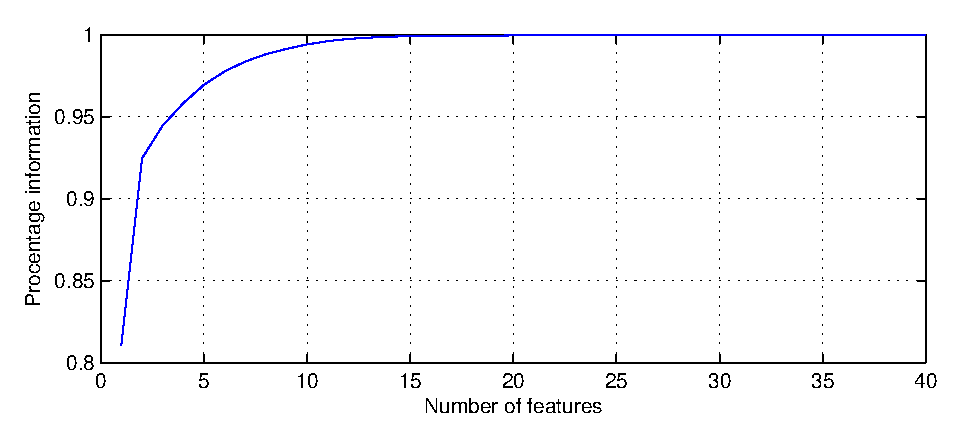
\includegraphics[width=\linewidth]{PCA_dist_var}
\caption{Cumulative distribution of variance (information) in dimensions sorted by highest eigenvalue}
\label{fig:PCA_dist_rap}
\end{figure}

Figure \ref{fig:PCA_dist_rap} shows cumulative distribution of variance in the separate dimensions of the feature space.
In this it is apparent most of the variance is contained within the first 5-10 dimensions. 
$ 94.9 \% $ at 5 dimensions and $ 99.4 \% $ at 10 dimensions.
This does not necessarily imply that most of the information is contained within these, but is a good indicator of this.

In this we see that truncating the feature space to one quarter of the dimensions (10) after PCA, has a very little effect on the overall accuracy of the classification.
This is important, since it can allow the classification algorithms to run with a much lower computational load.
 % DONE

	\section*{Probabilistic Generative Models}
This part of the article, describes the Probabilistic Generative models (PGM).
The assumed probabilistic model for each class is a multivariate normal distribution. 
\begin{equation}
p(\mathbf{x}|C_k)=
\mathcal{N}(\mathbf{x};\mathbf{\mu}_k, \; \Sigma_k) 
\label{eq:gauss_dist} 
\end{equation}

\paragraph*{Training}
In the training process the mean vector and covariance matrix of each class is estimated.
\begin{eqnarray}
\bm{\mu}_i= \dfrac{1}{N} \sum_{j=1}^{N} \mathbf{x}_{kj} \\
\bm{\Sigma}_k =\dfrac{1}{N} \sum_{j=1}^{N} (\mathbf{x}_{kj}-\bm{\mu}_k) \cdot (\mathbf{x}_{kj}-\bm{\mu}_k)
\end{eqnarray}
The mean and covariance from the training is used to calculate the probability density for each class.
\begin{equation}
p(\mathbf{x}|C_k)=  
\dfrac{1}{(2\pi)^{D/2}} \dfrac{1}{\left|\mathbf{\Sigma} \right|^{1/2}} 
\mathtt{exp} \left\lbrace -\dfrac{1}{2} (\mathbf{x}-\mathbf{\mu}_k)^T \mathbf{\Sigma}^{-1} (\mathbf{x}-\mathbf{\mu}_k) \right\rbrace
\end{equation}

The class prior is selected as an equal likelihood for each class. The probability of a given feature vector $ \mathbf{x} $ being part of a class $ C_k $ is given by.
\begin{equation}
p(C_k |\mathbf{x}) =
\dfrac{p(\mathbf{x}|C_k) p(C_k)}
{\sum_j p(\mathbf{x}|C_j) p(C_j)}
\end{equation}

\paragraph*{Result}
The result of the linear classifier is a total accuracy of 62.7, 58.1 and 57.2 \% respectively for one, two and ten digits.  % DONE?

	%!TEX root = Main.tex
\section*{Artificial Neural Networks}

The overall network function for a two layer neural network, takes the form
\begin{equation}
y_k(\mathbf{x},\mathbf{w}) = \sigma \left( \sum_{j=1}^{M} w_{kj}^{(2)} h\left( \sum_{i}^{D} w_{ji}^{(1)} x_i + w_{j0}^{(1)} \right) + w_{k0}^{(2)} \right) 
\label{eq:ANN_overall_rap}
\end{equation}

\subsection*{Training}
In the training of the neural network for a multi-class classification problem the following error-function is minimized.
\begin{equation}
E(\mathbf{w}) = \dfrac{1}{2} \sum_{n=1}^{N}\| \mathbf{y}(\mathbf{x}_n,\mathbf{w})-\mathbf{t}_n \|^2+\lambda| \mathbf{w}^T \cdot \mathbf{w}|
\label{eq:ANN_error_rap}
\end{equation}



\subsection*{Results}
The result of the ANN is a total accuracy of 95.3, 93.1 and 89.4 \% respectively for one, two and ten digits. 
The overall accuracy of the ANN model is very good, and the model can be used as an reliable speaker recognition classifier.  


	\section*{Gaussian Mixture Models}
Gaussian Mixture Models (GMM) is a way of finding and describing sub-populations in clusters of data points.
It is done by fitting a specified number of Gaussian distributions to a population of data points.
Each distribution is a component of the model. 
The individual data points are then arranged into clusters based on which model component is most likely given the observed data point.

The distributions of the mixture model are fitted to data by iteratively employing Expectation Maximization (EM).

\paragraph*{Training}
A GMM was trained for every speaker.
Then, for each speaker, a GMM is fitted to the respective speakers' training data, using MATLAB's Statistics Toolbox.

\paragraph*{Result}
The result of the GMM is a total accuracy of 94.6, 91.2 and 89.1 \% respectively for one, two and ten digits. 

	\section*{Support Vector Machines}
In this section the soft margin support vector machine (SVM) is described. 
The SVM is a binary classifier, which is a problem with multi class. 
The solution for multiclass classification is using a one-vs.-one setup.
The decision function for a standard SVM for a test point $ x_{new} $ is given by
\begin{equation}
t_{new} = \mathtt{sign}(\mathbf{w}^T \mathbf{x}_{new} +b)
\label{eq:SVM_lin}
\end{equation}

\paragraph*{Training}
The parameter vector $ \mathbf{w} $ is found by maximizing the margin or minimizing the length of the parameter vector, because of the inverse relationship $ \gamma = \frac{1}{\|\mathbf{w}\|} $.
In the training process of a soft margin SVM, the following expression is minimized. 
\begin{align}
\mathbf{w}^* = 
\mathtt{argmin}_\mathbf{w} \frac{1}{2} \mathbf{w}^T \mathbf{w}+C \sum_{n=1}^{N} \xi_n,\\ \mathtt{w.r.t.} \qquad t_n(\mathbf{w}^T \mathbf{x}_n + b) \geq 1-\xi_n
\end{align} 
The influence of each training point in the decision boundary is proportional to $ \alpha_n $.
After the training process, the classification can be done by using the following expression, where $ \mathbf{x}_n $  are the support-vectors, and $ \alpha_n $ is their weights.
\begin{equation}
t_{new} = 
\mathtt{sign}\left( \sum_{n=1}^{N} \alpha_n t_n k(\mathbf{x}_n,\mathbf{x}_{new}) +b  \right)
\end{equation}
with $ k = \mathtt{exp}(-\gamma \|\mathbf{x}^T_n - \mathbf{x}_{new} \|^2 ) $, which is the Gaussian kernel.

\paragraph*{Result}
The result was obtained by using a Gaussian kernel, and the classification accuracy was found to be 73.7 \% for the one digit dataset after training on the training set and afterwards classifying the test set.

\section*{Discussion}
This section contains a brief discussion of the results of the five different classification methods which have been used throughout this project. 

\begin{table}[h]
\begin{tabular}{@{}l|lll@{}}
\toprule
Model 		   		   & One digit            & Two digits  & Ten digits   \\ \midrule
ANN                    & 95.3 \%                & 93.1 \%   & 89.4 \% \\
GMM                    & 94.6 \%                & 91.2 \%   & 89.1 \% \\
SVM                    & 73.7 \%                & - 	    & -       \\ 
Linear                 & 55.9 \% 				& 51.2 \%   & 50.6 \% \\
PGM                    & 62.7 \% 				& 58.1 \%   & 57.2 \%
\end{tabular}
\caption{The accuracy of the model used in this project. \fxnote{hvis der kommer flere metoder skal den opdateres}}
\label{table:result}
\end{table}


\section*{Conclusion}


\bibliographystyle{ieeetr}
\renewcommand{\bibname}{2 Reference Document}
\addcontentsline{toc}{chapter}{2 Reference Document}
\bibliography{Appendix/10731@post.au.dk-RefList}



\end{document}
